\chapter{OpenStack}
\label{chap:OpenStack}


Minimal requirements
\begin{enumerate}
  \item 6 machines: one control node, one network node, one/many compute node,
  one/many block storage node, one/many object storage node.
  
  \url{http://docs.openstack.org/juno/install-guide/install/apt/content/ch_overview.html#example-architecture-with-neutron-networking-hw}
  
  \item 
\end{enumerate}

The selection of OS (Sect.\ref{sec:OpenStack_host-OS}) and hypervisor
(Sect.\ref{sec:hypervisor}) has a significant impact on the overall design and
also affects server hardware selection.
Ensure that the storage hardware is supported by the selected operating system
and hypervisor combination and that the networking hardware selection and
topology will work with the chosen operating system and hypervisor combination. 
\url{http://docs.openstack.org/arch-design/content/operating-system-and-hypervisor-arch-storage.html}


%Next is the hypervisor (Sect.\ref{sec:hypervisor}).

\section{Structure}

To design, deploy, and configure OpenStack, administrators must understand the
logical architecture. There are different modules, each one is one of the
following types

\begin{enumerate}
  \item daemon: run as a background process (on Linux platform) and is installed
  as a service
  
  \item script: is used to install a virtual environment as needed and run unit
  tests on a service
  
  \item CLI : a command-line interface that enables user to submit API calls to
  OpenStack daemons through easy-to-use commands
  
  \item 
\end{enumerate}


\begin{figure}[hbt]
  \centerline{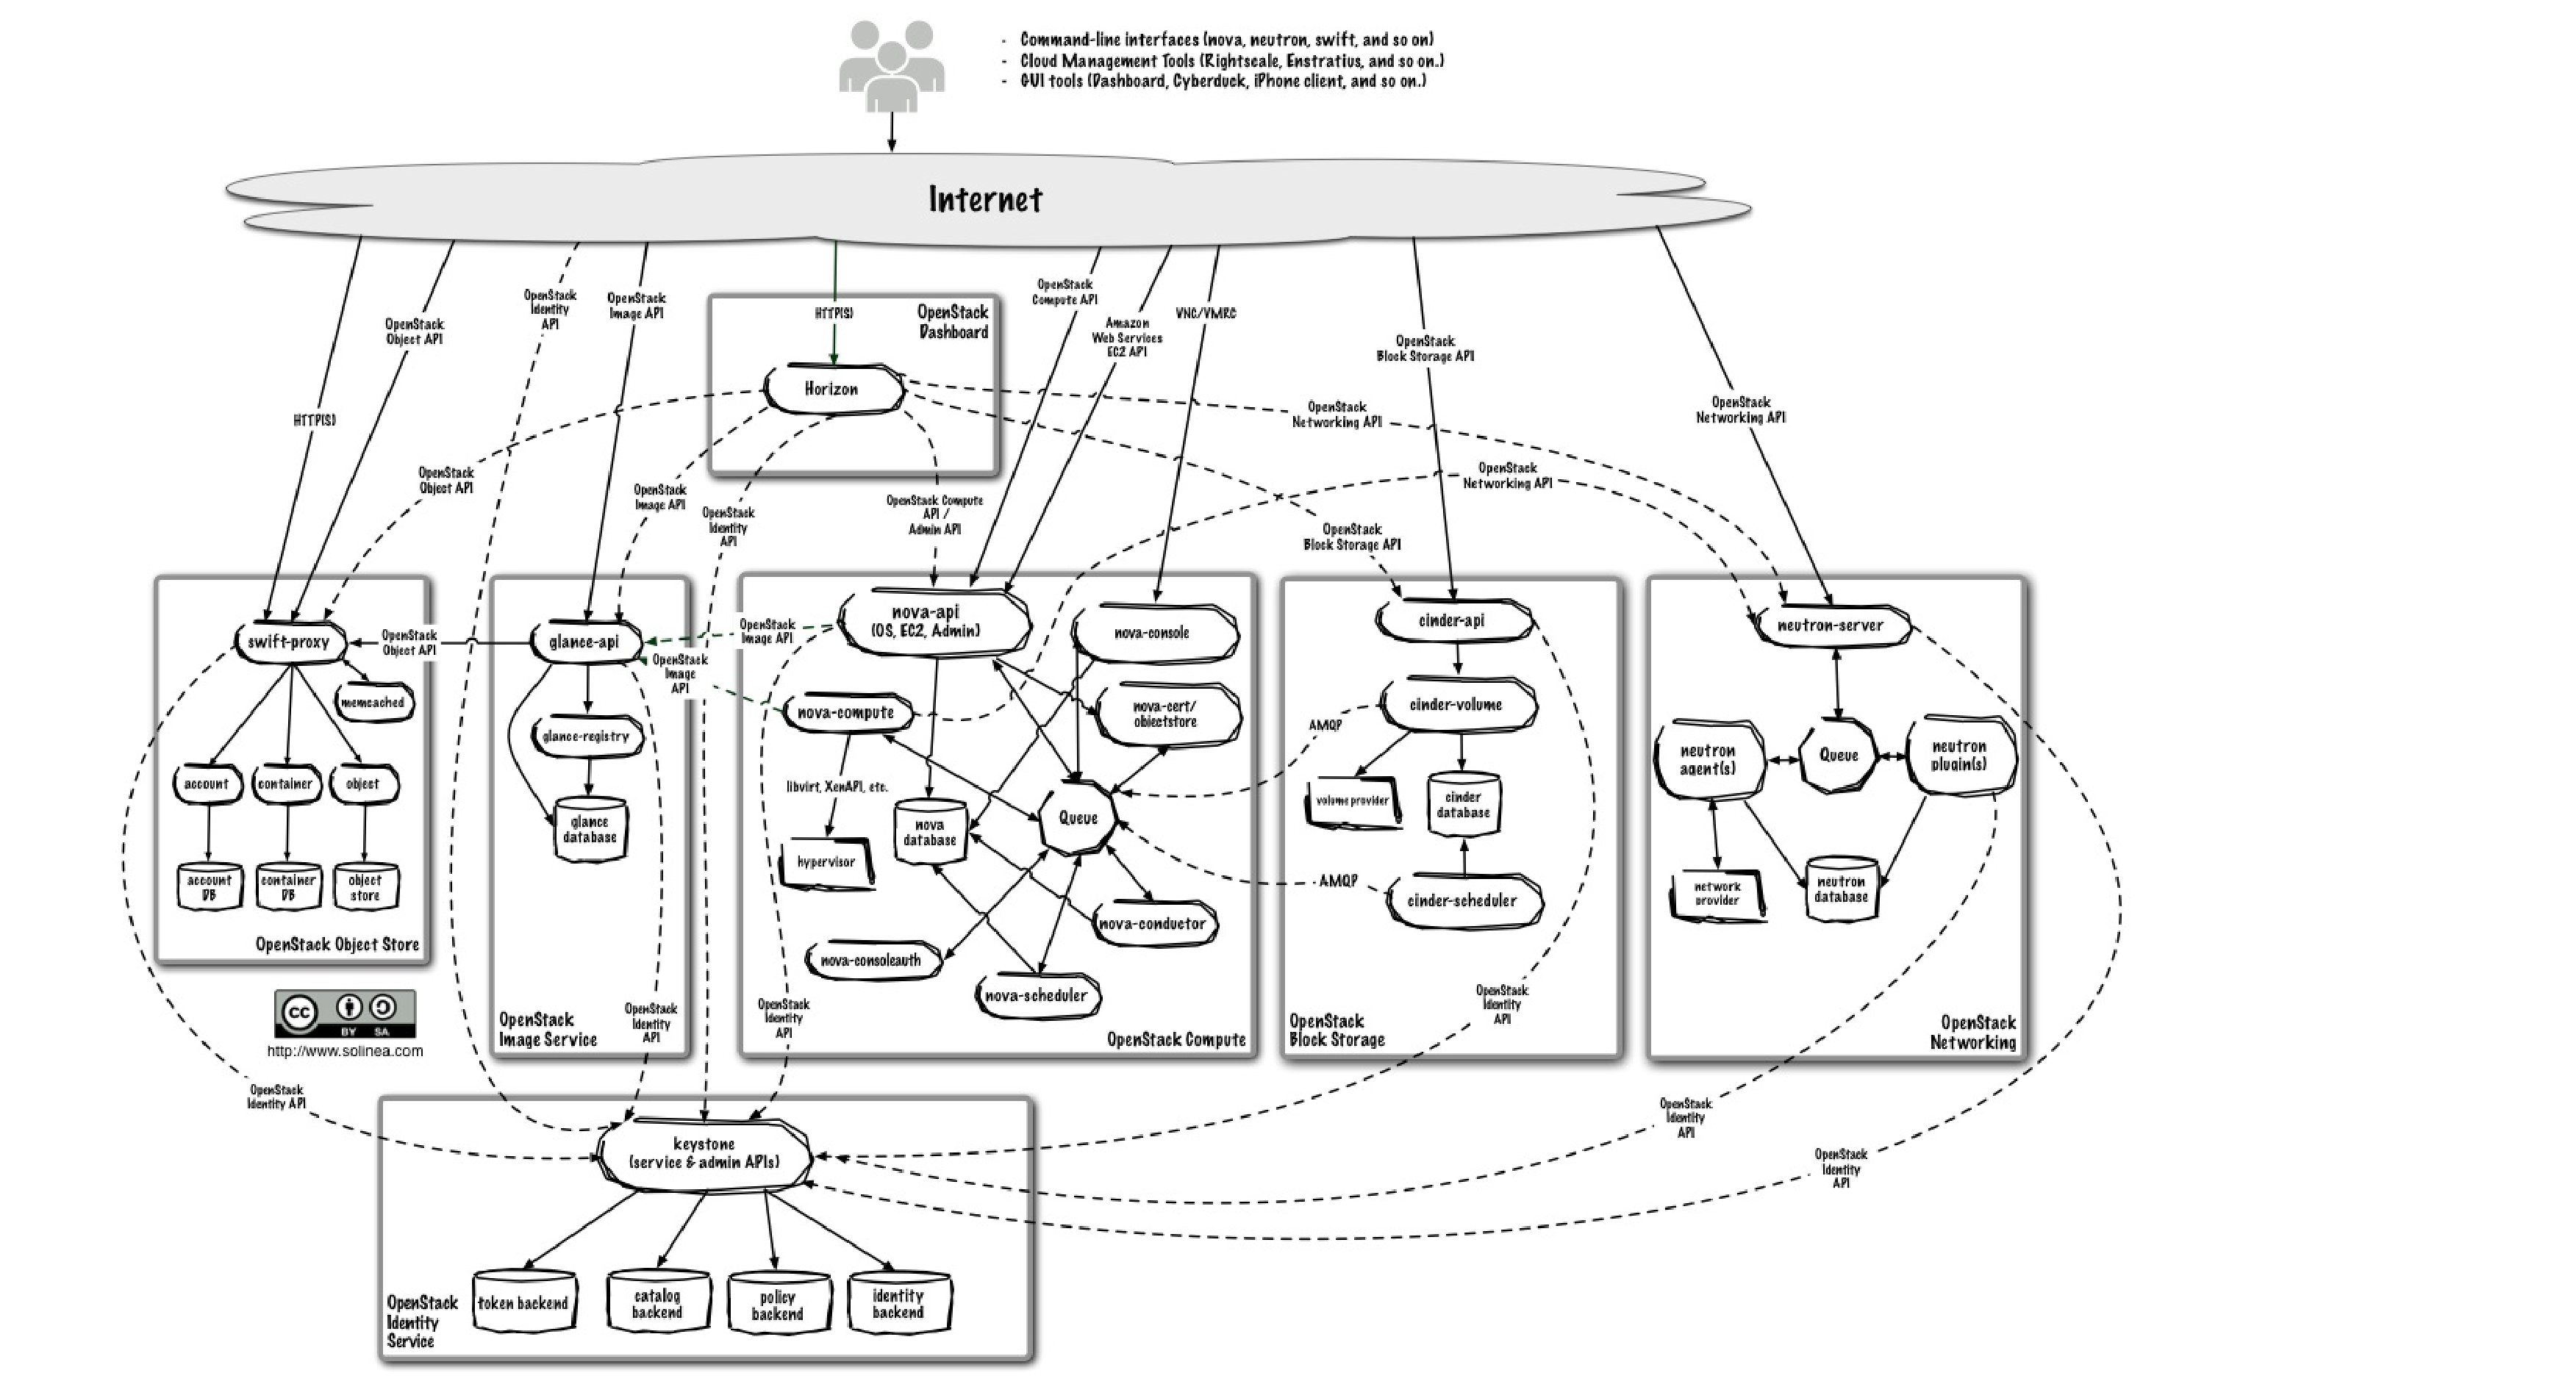
\includegraphics[height=3cm,
    angle=0]{./images/OpenStack_structure.eps}}
  \caption{Restitution curve
  \footnote{\url{http://www.physio.unibe.ch/~kucera/group/projects.aspx}}}
  \label{fig:OpenStack_structure}
\end{figure} 


There are basically eleven components of OpenStack, each one offers an API that
facilitates this integration.
\begin{enumerate}
  \item service Dashboard: project Horizon
  \item service Compute: project Nova
  \item service Networking: project Neutron
  \item service Object Storage: project Swift
  \item service Block Storage: project Cinder
  \item service Identity: project Keystone
  \item service Telemetry: project Ceilometer
  \item service Orchestration (automated arrangement, coordination, and
  management of complex computer systems, middleware, and services): project Heat
  
  Canonical use project Juju on Ubuntu O/S. Juju allows you to instantly deploy,
  integrate and scale your IT stack/services/applications.
  
  \item service Database Service: project Trove
\end{enumerate}

\section{Versions}

OpenStack releases are numbered YYYY.N time-based scheme, e.g. the second
release in 2012 will be 2012.2. There are also codename to identify the release,
with order alphabetically, e.g. Juno = the 10-th release so far. 
\url{https://wiki.openstack.org/wiki/Release_Naming}

\subsection{Austin}

\subsection{Bexar}

\subsection{Cactus}

\subsection{Diablo}

\subsection{Essex}

\subsection{Folsom}

\subsection{Grizzly}

\subsection{Havana}

\subsection{Icehouse}

\subsection{Juno}

OpenStack 2014.2 is Juno, the 10th release with 342 new features to support
\url{https://wiki.openstack.org/wiki/ReleaseNotes/Juno}
\begin{itemize}
  \item software development
  \item big data analysis
  \item application infrastructure at scale
\end{itemize}

\url{http://www.openstack.org/software/juno/}
\subsection{Kilo}


\section{host O/S}
\label{sec:OpenStack_host-OS}

Ubuntu is currently the most popular host O/S for OpenStack.
\footnote{\url{http://www.zdnet.com/article/openstacks-top-operating-system-ubuntu-linux/}}

To minimize clutter and provide more resources for OpenStack, we recommend a
minimal installation of your Linux distribution, with a 64-bit version on at
least the compute node (otherwise, we can not run 64-bit server instances of
guest O/S).
\url{http://docs.openstack.org/juno/install-guide/install/apt/content/ch_basic_environment.html}

You can install on a virtual machine, i.e. nested VM
(Sect.\ref{sec:OpenStack_single-node}), or a cluster
(Sect.\ref{sec:OpenStack_cluster}). OpenStack requires Ubuntu Server
\url{https://ask.openstack.org/en/question/4882/how-can-i-install-openstack-on-ubuntu-1204-desktop/}.
If we need the UI, we can install the UI later on Ubuntu Server.


\subsection{Cluster}
\label{sec:OpenStack_cluster}

The minimum amount of server is 7 with 2 disks, two of which have 2 NIC's.
Another option is to use Virtual MAAS.
\url{http://www.ubuntu.com/download/cloud/install-ubuntu-openstack}

\subsection{Single node}
\label{sec:OpenStack_single-node}

Ubuntu 12.04 running on Oracle VirtualBox with two NIC's.

\url{http://ilearnstack.com/2013/04/26/setting-up-a-single-node-openstack-environment/}



